%standard 14.2

%start_of_questions




%new_question
%%%%%%%%%%%%%%%%%%%%%
	% Problem 5
	% Difficulty: 2
%%%%%%%%%%%%%%%%%%%%%
	\item 
		A local middle school is trying to count the total number of lunches they served last year.  
		They have a text file named \textit{LunchData.txt} that has a date and the number of lunches served on that date.    
		There is one entry for every day last year.  A portion of that file is displayed below.  
		Write a program that calculates and then prints the total number of lunches served last year. 
		\begin{flushright}
			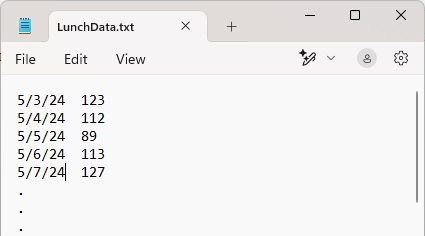
\includegraphics[scale=.65]{imgs/LunchData.PNG}
		\end{flushright}




%new_question
%%%%%%%%%%%%%%%%%%%%%
	% Problem 7
	% Difficulty: 2
%%%%%%%%%%%%%%%%%%%%%
	\item 
		A city library keeps track of the number of visitors each day in a file named 
		\textit{LibraryVisitsData.csv}.  
		The file contains a date and the number of visitors who entered the library on that date.  
		There is one entry for each day of the year. A portion of that file is shown below.  
		Write a program that reads the file, calculates, and prints the average number of visitors 
		per day over the year.
		
		\begin{flushright}
			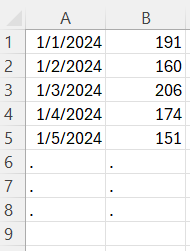
\includegraphics[scale=.65]{imgs/LibraryVisitsData.PNG}
		\end{flushright}


%new_question
%%%%%%%%%%%%%%%%%%%%%
	% Problem 8
	% Difficulty: 2
%%%%%%%%%%%%%%%%%%%%%
	\item 
		A local gym keeps a log of how many calories were burned in workout sessions each day, stored in a file called \textit{CaloriesBurnedData.txt}.  
		Each line of the file includes the date and the total number of calories burned by all gym members on that day.  
		A portion of the file is shown below.  
		Write a program that reads the file and prints the day with the highest number of calories burned.
		
		\begin{flushright}
			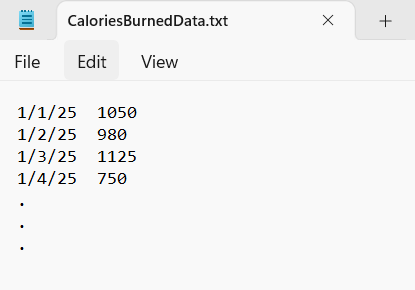
\includegraphics[scale=.65]{imgs/CaloriesBurnedData.PNG}
		\end{flushright}


%new_question
%%%%%%%%%%%%%%%%%%%%%
	% Problem 9
	% Difficulty: 2
%%%%%%%%%%%%%%%%%%%%%
	\item 
		A school science fair recorded the daily number of students who visited each exhibit. 
		This information is stored in a file called \textit{ScienceFairVisitors.txt}, which includes 
		a header row. Each line contains the date and the number of visitors for that day. 
		Write a program that reads the file, and then prints the total number of visitors recorded 
		over the entire period.
		
		\begin{flushright}
			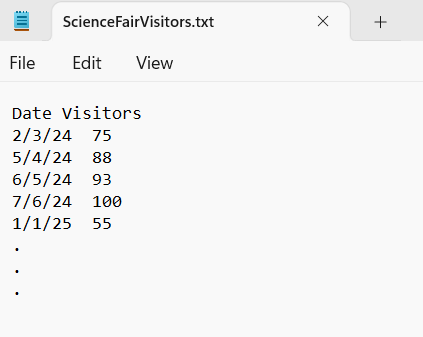
\includegraphics[scale=.65]{imgs/ScienceFairVisitorsData.PNG}
		\end{flushright}


%new_question
%%%%%%%%%%%%%%%%%%%%%
	% Problem 10
	% Difficulty: 2
%%%%%%%%%%%%%%%%%%%%%
	\item 
		A book club tracks how many pages each member read, stored in a file named 
		\textit{PagesRead.csv}. The file includes a header row and contains the member's 
		name and the number of pages they read for each book.  
		Write a program that reads the file, stores the data in a dictionary where the key is 
		the member name and the value is the total pages read by that member (across both books), 
		and then prints each member's name and their total pages read.
		
		\begin{flushright}
			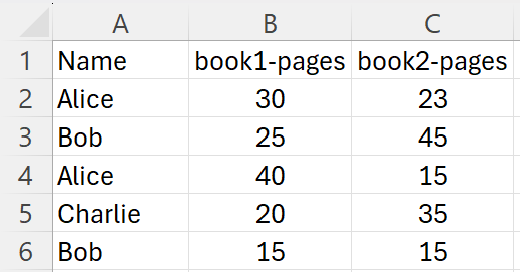
\includegraphics[scale=.65]{imgs/PagesReadData.PNG}
		\end{flushright}


%new_question
%%%%%%%%%%%%%%%%%%%%%
	% Problem 11
	% Difficulty: 2
%%%%%%%%%%%%%%%%%%%%%
	\item 
		A music streaming app tracks how many times each user listens to different songs.  
		The data is stored in a file called \textit{SongPlays.txt}, which includes a header row.  
		Each line contains the user’s name and the number of times they played a song on a given day.  
		Write a program that reads the file, uses a dictionary to store the total plays per user, 
		and then prints out each user and their total number of song plays.
		
		\begin{flushright}
			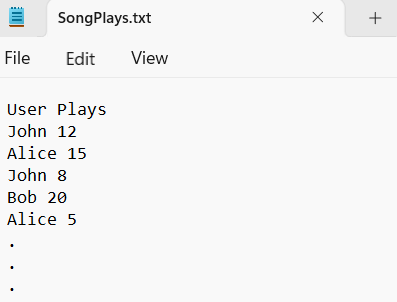
\includegraphics[scale=.65]{imgs/SongPlaysData.PNG}
		\end{flushright}


%new_question
%%%%%%%%%%%%%%%%%%%%%
	% Problem 12
	% Difficulty: 2
%%%%%%%%%%%%%%%%%%%%%
	\item 
		A weather station logs the temperature each day and stores the data in a file called 
		\textit{DailyTemperatures.csv}. The file includes a header row and each line contains the date 
		and the temperature recorded on that day. Write a program that reads the file, stores all the 
		temperatures in a list, and then prints the highest, lowest, and average temperature recorded.
		
		\begin{flushright}
			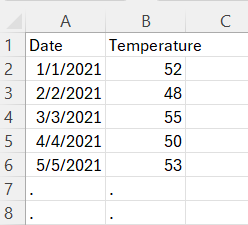
\includegraphics[scale=.65]{imgs/DailyTemperaturesData.PNG}
		\end{flushright}


%end_of_questions
%make sure to leave at least one blank line below

